
\chapter{Material und Methoden}\label{method}


\section{Material}\label{material}
Als Material zu Verfügung stehen instesammt 86 Patient*innen als Datensatz. Die dazugehörigen Grade der House-Brackmann Skala, sind hierbei nicht gleichverteilt vorhanden. Der Grad VI ist prozentual ungefähr im gleichen Maße vorhanden wie die Grade I-V zusammen (Abb. \ref{cap:pie_grade}). Der Grad I ist nur mit einem Patient*in vertreten.

\begin{figure}[!b]\centering
\begin{tikzpicture}
\pie[sum=auto, radius=2.45, text=pin]{1/I , 6/II, 9/III, 22/IV, 8/V, 40/VI }
%\pie[pos ={10,0}, sum=auto, radius=3.5, text=legend]{1/I , 6/II, 9/III, 22/IV, 8/V, 40/VI }
\end{tikzpicture}
\caption[Verteilung der einzelnen Grade der House-Brackmann Skala]{Verteilung der einzelnen Grade der House-Brackmann Skala des zu Verfügung stehenden Datensatzes. Klar erkennbar ist das ungleiche Vorhandensein der Grade.}\label{cap:pie_grade}
\end{figure}\label{fig:pie_grade}


 Jeder Patient*in inkludiert 9 verschiendene Bilder, die verschiedenste Posen darstellen. Die Gesichtsausdrücke in den Einzelbilder können jeweils einen kontreten Teil des House-Brackmann Scores zugeordnet werden. Zudem werden die normalerweise in Bewegung stattfindenden Ausdrücke statisch im Bild eingefangen. Die Bildcoderung (Posendarstellung) dieser 9 Bilder lautet:

\begin{enumerate}
  \setlength\itemsep{-0.6em}
\item Ruhender Gesichtsausdruck
\item Augenbrauen heben
\item Lächeln, geschlossener Mund
\item Lächeln, geöffneter Mund
\item Lippen schürzen, \glqq Duckface\grqq{}
\item Augenschluss, leicht
\item Augenschluss, forciert
\item Nase rümpfen
\item Depression Unterlippe
\end{enumerate}

Das Bild mit der Codierung 1 fokusiert sich dabei auf die Symmetrie in Ruhe. Die 2 bildet die Stirn ab. Dadurch sollen die Auswirkungen und die Beweglichkeit der Muskeln rund um die Stirnpartie gezeigt werden (absichtliche Faltenbildung). Der Lidschluss wird mit den Bildern 6 und 7 statisch eingefangen. Meistens ist ein nicht geschlossenes Auge durch das Weiße im Augenball erkennbar. 3, 4, 5, 8 und 9 zeigen den Mund in unterschiedlichtsen Positionen.

Problematisch dabei ist, dass nicht für jeden Patient*in alle 9 korrespondierenden Bilder vorhanden sind (Abb. \ref{cap:bar_code}).


\begin{figure}[!tb]\centering
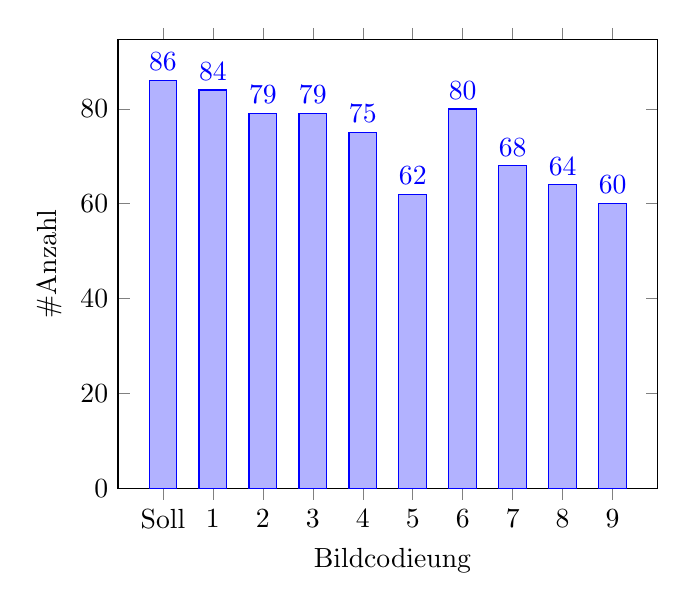
\begin{tikzpicture}
\begin{axis}
[
    ybar,
    ymin=0,
    %enlargelimits=0.15,
    ylabel={\#Anzahl}, % the ylabel must precede a # symbol.
    xlabel={\ Bildcodieung},
    symbolic x coords={Soll, 1, 2, 3, 4, 5, 6, 7, 8, 9},
    xtick=data,
    nodes near coords, % this command is used to mention the y-axis points on the top of the particular bar.
    nodes near coords align={vertical},
    ]
\addplot coordinates {(Soll,86) (1,84) (2,79) (3,79) (4,75)
                      (5,62)    (6,80) (7,68) (8,64) (9,60) };

\end{axis}
\end{tikzpicture}
\caption[Anzahl der vorhandenen  Einzelbilder aller Patient*innen]{Anzahl der vorhandenen  Einzelbilder aller Patient*innen. Der Sollwert beträgt 86 für alle.}\label{cap:bar_code}
\end{figure}\label{fig:bar_code}








\clearpage
\section{Modulverarbeitung}\label{module}
\textbf{TODO, Anpassung der House-Brackmann Skala hier migirieren, Zerschneigung des Gesichtes, erklärung der Einzelmodule}

Für die Detektion des Grades nach House-Brackmann, werden die einzelnen Merkmale der Skala in Module eingeteilt (Abb. \ref{cap:module_graph}). Ziel dieser Aufteilung ist es Expertensysteme für die Teilbereiche der House-Brackmann Skala zu bilden. Diese muss für die Detektion angepasst werden. Die dynamischen Eigenschaften Stirn, Lidschluss und Mund können so nicht als ein Label interpretiert werden. Die 9 Eingabebilder in das System stellen die Posen statisch dar. So können alle Eigenschaften bis auf Lidschluss nach der House-Brackmann Skala auf die Grundlabel Normal, minimale Asymetrie, Asymmetrie und Keine reduziert werden. Lidschluss besitzt nurnoch die zwei Möglichkeiten, vollständig geschlossen oder geöffnet zu sein (Tabelle \ref{cap:housebrackmannnew}).
Nach dieser Tabelle werden so für die einzelnen Module die passenden Label bestimmt.

\begin{table}[h]\vspace{1ex}\centering
  \begin{tabular}{c||c|c|c|c|}
  Grad & Symmetrie    & Stirn  & Lidschluss    & Mund         \\ \hline\hline
  I    & Normal       & Normal & Vollständig   & Normal       \\ \hline
  II  & Normal & Normal                                                        & Vollständig & \begin{tabular}[c]{@{}c@{}}minimale\\ Asymmetrie\end{tabular} \\ \hline
  III & Normal & \begin{tabular}[c]{@{}c@{}}minimale\\ Asymmetrie\end{tabular} & Vollständig & \begin{tabular}[c]{@{}c@{}}minimale\\ Asymmetrie\end{tabular} \\ \hline
  IV   & Normal       & Keine  & Unvollständig & Asymmetrisch \\ \hline
  V    & Asymmetrisch & Keine  & Unvollständig & Asymmetrisch \\ \hline
  VI   & Keine        & Keine  & Unvollständig & Keine        \\ \hline
  \end{tabular}
  \caption[Angepasste House-Brackmann Tabelle zur Bestimmung der Label]{Angepasste House-Brackmann Tabelle zur Bestimmung der Label}\label{cap:housebrackmannnew}
\vspace{2ex}\end{table}\label{table:housebrackmannnew}



\begin{figure}[!tb]\centering
\begin{tikzpicture}[->,>=stealth',shorten >=1pt,auto,node distance=2.5cm,semithick]
  \tikzstyle{every state}=[fill=cyan,draw=black,text=black]

  \tikzstyle{level1} = [rectangle, draw, fill=green!40!blue!20, text width=8cm, text centered, inner sep=1pt  , minimum height=1.3cm]
  \tikzstyle{level2} = [rectangle, draw, fill=blue!20,          text width=2cm, text centered, rounded corners, minimum height=2.5cm]
  \tikzstyle{level3} = [rectangle, draw, fill=green!40!blue!20, text width=8cm, text centered, inner sep=1pt  , minimum height=1.3cm]
  \tikzstyle{level4} = [rectangle, draw=white, fill=white, text width=1cm, text centered, minimum height=0.1cm, minimum width=0.1cm]

  \tikzstyle{container} = [draw, rectangle, dashed, inner sep=8pt, minimum width=15cm]

  \node[level4]         (Z1)                                 {};

  \node[level1]         (A) [left of=Z1, xshift=8cm]        {Regions of Interest};
  \node[level2]         (B) [below left  of=A, yshift=-2cm] {Lidschluss};
  \node[level2]         (C) [below right of=A, yshift=-2cm] {Mund};
  \node[level2]         (D) [left  of=B]                    {Symmetrie};
  \node[level2]         (E) [right of=C]                    {Stirn};
  \node[level3]         (F) [below right of=B, yshift=-2cm] {Fusionierung};
  \node[container, fit=(B) (C) (D) (E)] (his) {};
    \node at (his.north west) [below right,node distance=0 and 0] {Module};

  \node[level4]         (Z2) [right of=F, xshift=3cm]        {};

  \path (Z1) edge [out=0   , in=180] node [left, xshift=-0.3cm]                {Input $x$} (A)

        (A) edge [out=-145, in=90 ] node [right, yshift=-0.1cm, xshift=0cm   ] {$x_{l}$} (B) %Lidschluss
            edge [out=-35 , in=90 ] node [left , yshift=-0.1cm, xshift=0cm   ] {$x_{m}$} (C) %Mund
            edge [out=-160, in=90 ] node [above, yshift=-0.5cm, xshift=0.8cm ] {$x_{s}$} (D) %Symmetrie
            edge [out=-20 , in=90 ] node [above, yshift=-0.5cm, xshift=-0.5cm] {$x_{f}$} (E) %Stirn
        (B) edge [out=-90 , in=145] node [right, yshift=0.1cm , xshift=0cm   ] {$y_{l}$} (F)
        (C) edge [out=-90 , in=35 ] node [left , yshift=0.1cm , xshift=0cm   ] {$y_{m}$} (F)
        (D) edge [out=-90 , in=160] node [below, yshift=0.5cm , xshift=0.8cm ] {$y_{s}$} (F)
        (E) edge [out=-90 , in=20 ] node [below, yshift=0.5cm , xshift=-0.5cm] {$y_{f}$} (F)

        (F) edge [out=0   , in=180] node [right, xshift=0.3cm]                {Output} (Z2);

\end{tikzpicture}
\caption[Darstellung der Modulbauweise]{{Schematische Darstellung der Module}\label{cap:module_graph}}
\end{figure}\label{fig:module_graph}

Anhand von Markerpunkten im Gesicht sollen die 9 Bilder jeder Patient*in in die Bestandteile der Skala, in die Regions of Interest, zerschnitten werden, um nur die jeweils relevanten Teile zu betrachten um proaktiv zu verhindern, dass die Neuronalen Netze nicht notwendige Eigenschaften betrachten. Zu den nicht notwendigen Bestandteile des Bildes zählen Hintergrund, welches verschiedenste Farben und Helligkeitsstufen annehmen kann und der Körper des Patient*innen. Nur der Kopf ist für die Feststellung der Parese nötig. Die Landmarks, die für die Einteilung in die Regionen müssen dazu immer an der selben Position $P$ im Array sein (Abb. \ref{cap:abba}). Nach der Formel (\ref{eg:bbox}) und der jeweils zugeordneten Punkte, können die Eingabebilder für die Module definerit werden (Tabelle \ref{cap:rel_landmarks}). Dabei sind $a_{min}, b_{min}$ und $a_{max}, b_{max}$ die beiden neuen Ecken.

\noindent\begin{minipage}{.5\linewidth}
\begin{alignat*}{3}
  a_{min} &= min(P[:, 0]) &\quad &\textrm{| Extrema links}\\
  a_{max} &= max(P[:, 0]) &\quad &\textrm{| Extrema rechts}\\
  b_{min} &= min(P[:, 1]) &\quad &\textrm{| Extrema oben}\\
  b_{max} &= max(P[:, 1]) &\quad &\textrm{| Extrema unten}
\end{alignat*}
\end{minipage}%
\begin{minipage}{.5\linewidth}
  \begin{equation}
  \begin{split}
    &\textrm{Bedingungen:}\\
    &\textrm{1.}\quad  a_{min} < a_{max}\\
    &\textrm{2.}\quad  b_{min} < b_{max}\\
    &\textrm{3.}\quad a_{min}, a_{max}, b_{min}, b_{max} \in \mathbb{N}
  \end{split}
  \label{eg:bbox}
  \end{equation}
\end{minipage}

\vspace{1cm}

Die Box spannt einen Raum auf, dessen Inhalt das Eingabebild für eines der Module (z.B Lidschluss nur Punkte $P(36)$ bis $P(47)$) relevant ist. Alles was sich nicht innerhalb des Rechteckes befindet wird weggeschnitten. Ein Offset wird dazu noch in alle Richtungen addiert bzw. subtrahiert um Ungleichheiten in der Landmarkberechnung auszugleichen.








\begin{table}[!tb]\vspace{1ex}\centering
\begin{tabular}{c||c|c}
Modul & \begin{tabular}[c]{@{}c@{}}zugeschnittenes\\ Eingabebild\end{tabular} & \begin{tabular}[c]{@{}c@{}}Betrachtete\\ Landmarks\end{tabular} \\ \hline\hline
Symmetrie  & $x_s$  & P(00) - P(68)  \\ \hline
Lidschluss & $x_l$  & P(38) - P(47) \\ \hline
Mund       & $x_m$  & P(48) - P(68) \\ \hline
Stirn      & $x_f$  & P(17) - P(27) \\ \hline
\end{tabular}
\caption[Zuordnung der Module zu die relevanten Punkte der Landmarks und das Eingabebild in die Module nach dem Ausschneiden vom Originalbild $x$]{Zuordnung der Module zu die relevanten Punkte der Landmarks und das Eingabebild in die Module nach dem Ausschneiden vom Originalbild $x$}\label{cap:rel_landmarks}
\vspace{1ex}\end{table}\label{fig:rel_landmarks}






\begin{figure}[t]\centering
%\resizebox{1.2\textwidth}{!}{
  %width=0.98\textwidth
\makebox[0pt]{\includesvg[inkscapelatex=false, width=30cm]{./images/landmarks}}
%}
\vspace{-1cm}
\caption[Abba]{TODO Regionen Einzeichnen, Framework nennen}\label{cap:abba}
\end{figure}\label{fig:abba}


Die einzelnen Module Symmetrie, Lidschluss, Mund und Stirn (Abb. \ref{cap:module_graph}) sind vortrainierte ResNet18 Netze vom ImageNet Contest. Benutzen von vortrainierte Netzen spart wertvolle Trainingszeit durch die an den Layern und schon vorhandenen Parameter. Diese einzelnen Gewichte an den Kanten müssen so nurnoch verfeinert werden, um damit das gewünschte Ergebnis zu erzielen. Für alle Experimente (siehe Kapitel \ref{experiment} Experimente) ist das gewählte Netz identisch, damit die Ergebnisse vergleichbar sind. Die Abbildungsvorschrift für die Relation Eingabebild $x$ mit der Pixelgröße $a, b$ und drei Schichten für den Farbraum RGB zu auszugebenden Label $y$ ist:

\begin{equation}
y: \mathbb{R}^{3 \times a \times b} \to \mathbb{R}, y(x) = resnet18(x)
\end{equation}

Jedem Eingabebild ist so genau eine natürliche Zahl zugeordnet. Diese Zahl ist letzenendes eine Nummer, die ein Label repräsentiert nach der oben genannten Tabelle. Die Operation liefert Wahrscheinlichkeiten für alle Label der Kategorie.

Im Anschluss nachdem alle Label der seperaten Module ausgerechnet wurden, können diese fusioniert werden um den Grad nach House-Brackmann zu bestimmen. Dabei gibt es zwei Vorgehensweisen, die Experimentell zu bestätigen sind (siehe Kapitel \ref{fusion}). Dabei können einmal alle Wahrscheinlichkeiten direkt als Zeilensumme gebildet werden. So kann direkt der am höchsten befindliche Wert einer Zeile der Tabelle den an der linken Seite befindlichen Grad angenommen werden. Eine andere Herangehensweise ist das heranziehen eines Automaten. Dazu werden zuerst die Wahrscheinlichkeiten in Label umgemünzt. Die Position des höchsten Wert im zurückgelieferten Array ist gleich der Position des Labels nach der Tabellenspalte. Alle Positionen jedes Modules durchlaufen den Automaten. Der Endzustand des Automaten, wenn alle Label jedes Modules den Automaten durchläuft, ist der zu ermittelnde Grad nach House-Brackmann.

















\clearpage
\section{Oversampling zum Klassenausgleich}\label{oversamplingmethod}
\textbf{TODO}

\section{Early Fusion und Late Fusion}\label{fusionmethod}
\textbf{TODO Early Fusion Concatenation}








\clearpage
\section{Caching}\label{caching}
\textbf{TODO: Problem schildern}


Zwei mögliche Lösungsansätze wären \ac{lru} und eine stationäre externe Datenbank als, der als temporären Cache agiert.

\subsection{Least Recently Used Cache}\label{lrucache}
\ac{lru}, bedetuet, der am längsten nicht zugegriffenen Eintrag wird aus dem Cache entfernt. Vergleichen lässt sich das mit einer Warteschlange mit begrenztem Platzinhalt. Aufgerufene Elemente reihen sich am Ende der Warteschlange ein (im dargestellten Array die linke Seite). Alle nachfolgenden wandern um eine Position nach vorne. Der Vorderste in der Warteschlange wird entfernt (Abb. \ref{cap:lrucache}), sobald ein noch nicht bekannes Element einreiht. Dieses neue Element muss zur Laufzeit initial berechnet werden. Danach ist es solange Verfügbar bis es wieder herausgeschoben wurde.

Einträge im Cache haben einen Index. Über diesen werden auf die dahinter liegenden Elemente zugegriffen. Sei $l$ die Länge des Caches und $\Sigma$ Indizes (z.B. A-Z). Insgesammt $l$ Elemente können im Cache für das schnelle Aufrufen vorgehalten werden.

\begin{figure}[h]\centering
\begin{tikzpicture}[->,>=stealth',shorten >=1pt,auto,node distance=4cm,semithick]

  \tikzstyle{style} = [rectangle, draw, fill=green!40!blue!20, text centered, inner sep=1pt  , minimum height=2cm, align=center]

  \node[style] (A)              {Cache\\ {[A,B,C,D,E]}};
  \node[style] (B) [right of=A] {Cache\\ {[\textbf{B},A,C,D,E]}};
  \node[style] (C) [right of=B] {Cache\\ {[\textbf{E},B,A,C,D]}};
  \node[style] (D) [right of=C] {Cache\\ {[\textbf{Z},E,B,A,C]}};

  \path (A) edge  node [yshift=-1cm, align=center] {B\\ \\ \textcolor{green}{Hit}} (B)
        (B) edge  node [yshift=-1cm, align=center] {E\\ \\ \textcolor{green}{Hit}} (C)
        (C) edge  node [yshift=-1cm, align=center] {Z\\ \\ \textcolor{red}{Miss}}  (D);

\end{tikzpicture}
\caption[Beispiel des \ac{lru}]{Beispiel des \ac{lru} mit $l=5$ und dem $\Sigma=A-Z$}\label{cap:lrucache}
\end{figure}\label{fig:lrucache}


Im Cache liegenden Elemente besizen eine kürzere Aufrufdauer als diejenigen, die nicht im Cache sind. Die \ac{wcet}, die Zeit welche benötigt wird um ein Element aufzufen, beträgt für

\begin{itemize}
\item im Cache liegende Elemente: $WCET_{ges}=WCET_{cache}$
\item nicht im Cache liegende Elemente: $WCET_{ges}=WCET_{cache} + WCET_{berechnung}$
\end{itemize}

Dabei ist $WCET_{cache}$ die Laufzeit, die für das Nachschauen der Elemente im Cache benötigt wird und $WCET_{berechnung}$ für die initiale Berechnung des abzuspeichernden Elementes beträgt. Solange $l$ nicht wesentlich kleiner als die Anzahl von Elementem im Dataloader ist, können teilweise Einträge wiederverwertet werden, wenn ein neuer Epoch in der Trainingsphase der Neuronalen Netze beginnt. Die Berechnung der recycelten Elemente kann so eingespart werden, woraus eine kürzere Laufzeit zu erwarten ist.






\subsection{Datenbank}\label{database}
Eine weitere Möglichkeit ist es, Elemente in eine relationale Datenbank zu speichern. Der Aufbau ist dabei relativ Identisch zu dem \ac{lru}. Über einen Index wird auf das benötigte Element zugegriffen, jedoch sind \textbf{alle} Elemente in der Datenbank gespeichert. Die \ac{wcet} beträgt immer die Zeit, welche zum Zugriff auf die Datenbank benötigt wird. Zusätzlich kommt die Rechenzeit hinzu, welche benötigt wird, um alle Elemente in die Datenbank einzutragen. Solange nicht auf den selben Index geschrieben wird, ist es ratsam die Einträge parallel in die Datenbank zu schreiben, um Rechenzeit zu sparen. Indexe müssen als Primärschlüssel einendeutig sein, damit keine Konflikte beim Schreiben und Lesen auftreten!

\begin{table}[h]\vspace{1ex}\centering
  \begin{tabular*}{9cm}{c|c}
  \textbf{Indizes (Primärschlüssel)} & \textbf{Elemente}
  \\\hline
  A   &  Bild 1 \\
  B   &  Bild 2 \\
  C   &  Bild 3 \\
  D   &  Bild 4 \\
  E   &  Bild 5 \\
  ... & ...

  \\\hline
  \end{tabular*}
  \caption[Beispieltabelle in einer relationalen Datenbank]{Beispieltabelle in einer relationalen Datenbank}\label{cap:database}
\vspace{2ex}\end{table}\label{table:database}


Vorteil dieser Methode ist es, die kurze Lesezeit von der Datenbank ($WCET_{read}$) auszunutzen, da diese kleiner ist als die Berechnung zur Laufzeit ($WCET_{berechnung}$). In der Trainingsphase werden $z$ Epochs durchlaufen. Dadurch werden statt  $WCET_{berechnung} * z$ nur $WCET_{read} * z$ Zeiteinheiten benötigt, wobei gilt $WCET_{berechnung} > WCET_{read}$. Dadurch kann die Trainingsphase schneller beendet werden.
































%\section{?Use Cases}\label{usecase}
% \paragraph{Definition:}
% Use Case Diagramme auch bekannt als „Anwendungsfalldiagramm“ werden verwendet, um das Verhalten des Systems aus Sicht der Benuter zu modellieren.
% Benuter (dargestellt als Strichmännchen) oder Systeme sind Akterue, die miteinander agieren, die den jeweiligen \Acp{uc} abbilden. Die jeweiligen Relationen zwischen Akteure und den \ac{uc} werden mit Linien verbunden. Möglich sind auch Verbingung zwischen \ac{uc}. Dabei können sie andere \ac{uc} optional Erweitern (extend) oder Inkludieren einen weiteren, der den Basis Use Case erweitert. Auch sind Generalisierungen (Vererbung) möglich. So werden alle Eigenschaften und Fälle auf die Spezialisierung übernommen. \textbf{TODO Quelle!!!}
%
%
% \paragraph{Use Cases des Experimentes (siehe Abb. \ref{cap:usecase}):}
% Nach Erfolgrecher Beendigung des Experimentes können die Anwendungsfälle definiert werden. Folgende Akterure kristallisieren sich aus den \ac{uc} heraus:
% \begin{itemize}
% \item Benutzer*innen (Benutzer*innen/Patient*innen, die eine Kategorisierung erwünscht)
% \item Administrator*innen (Verwalter des Systems)
% \item Docker Container (Instanz auf einem Server, der den Sourcecode laufen lässt und über eine Schnittstelle den Zugriff ernöglicht)
% \end{itemize}
%
% \begin{figure}[h]
% \begin{center}
%  \includesvg[width=0.98\textwidth]{./images/UseCase}
% \caption[Use Case Diagramm]{Anwendungsfälle des Experimentes als Use Cases beschrieben.}\label{cap:usecase}
% \end{center}
% \end{figure}\label{fig:usecase}
%
% Administrator*innen verwalten im allgemeinen das System. Diese führen die Trainingsphase aus und versuchen, so genau wie möglich, die Ergebnisse für den Hosue-Brackmann Grad, zu ermitteln. Dabei handelt sich es um ein Optimierungsproblem. Parameter können die Lernrate der Neuronalen Netze beeinfulssen. Auch welches Neuronale Netz zur Anwendung kommt wird von ihnen beeinflusst.
%
% Über einen API Zugriff können so Benutzer*innen für sich selbst die Detection starten indem sie über einen Request an den Server, der die Komponenten hostet, stellt. Dieser sendet ihnen nach der Berechnung das Ergebnis zurück. Im Hintergrund führt der Server, in dem Fall dargestellt als Docker-Container, der über eine IP-Adresse für die Aussenwelt erreichbar ist, die Berechnung aus.
%
%
% \begin{figure}[h]
% \begin{center}
%  \includesvg[width=0.98\textwidth]{./images/API_Request}
% \caption[Aktivitätsdiagramm eines schematischen Ablaufes eines  Requestes]{Aktivitätsdiagramm eines schematischen Ablaufes eines Requestes.}\label{cap:apirequest}
% \end{center}
% \end{figure}\label{fig:apirequest}
